% Generated by pysimcount.pffigure -- do not edit; regenerate instead.
% figure: B-order6-by-formula -- Every order-6 formula at measured r
% source: results/pf-thesis/results.json
% metric=total gatebase=cz merged
% seed=1 t=n template=simcount synth=pygridsynth
% git_commit=04cd66abb614bdc66fb48e891cef085a299e0ab1 git_dirty=False
% source_sha256=018e0b7603e6fc9f6ee358974f241415a3b93437700847b033937cc1d4250db8
% derived: B-order6-by-formula.tex restyled by pysimcount.figuniform: extrapolated points (r from power-law fit) drawn in their series' measured style, style-key legend entries removed; extrapolated n = [13, 20]; source_sha256=f1e49e2bd0bf3d72397c39543f47409e4e9fe9c8a4959e4f6499dd6c76e50d66
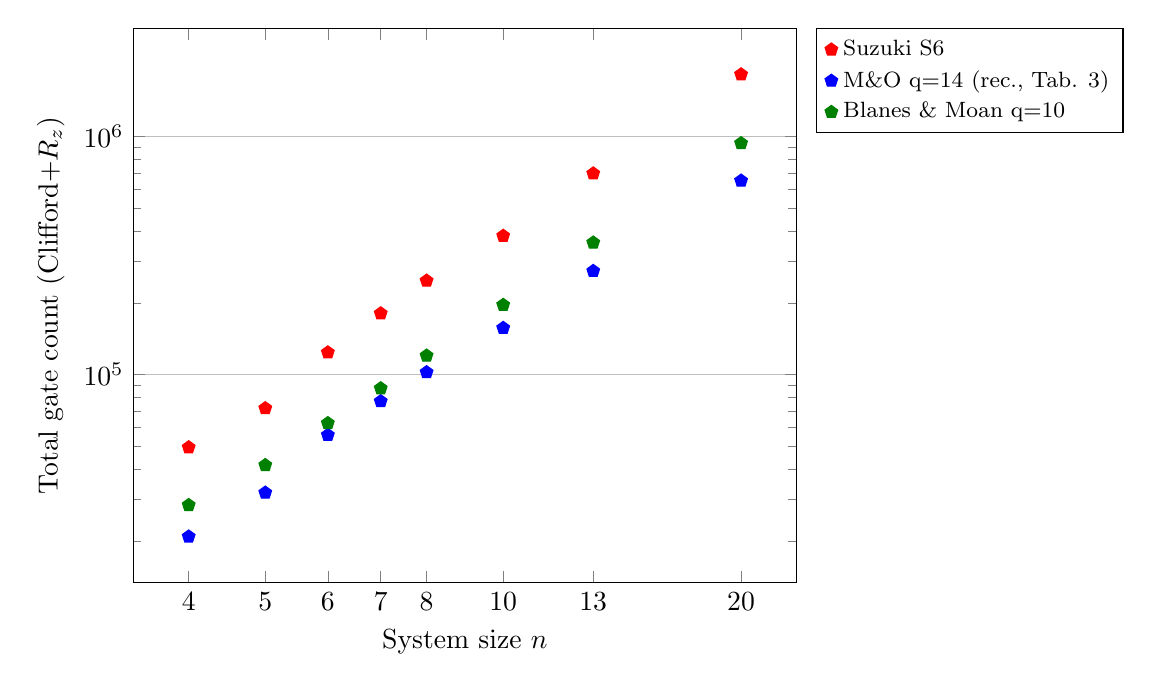
\begin{tikzpicture}
  \begin{loglogaxis}[
    width=10cm,
    xlabel={System size $n$},
    ylabel={Total gate count (Clifford+$R_z$)},
    xtick={4,5,6,7,8,10,13,20},
    xticklabels={4,5,6,7,8,10,13,20},
    ymajorgrids=true,
    legend pos=outer north east,
    legend cell align=left,
    legend style={font=\footnotesize},
  ]
    \addplot[only marks, red, mark=pentagon*, mark size=2.4pt, mark options={solid, fill=red}] coordinates {
      (4,49536)
      (5,72240)
      (6,123840)
      (7,180600)
      (8,247680)
      (10,381840)
    };
    \addlegendentry{Suzuki S6}
    % r from power-law fit (extrapolation); one legend entry per series
    \addplot[only marks, red, mark=pentagon*, mark size=2.4pt, mark options={solid, fill=red}, forget plot] coordinates {
      (13,697632)
      (20,1816320)
    };
    \addplot[only marks, blue, mark=pentagon*, mark size=2.4pt, mark options={solid, fill=blue}] coordinates {
      (4,20916)
      (5,31955)
      (6,55776)
      (7,77273)
      (8,102256)
      (10,156870)
    };
    \addlegendentry{M\&O q=14 (rec., Tab. 3)}
    % r from power-law fit (extrapolation); one legend entry per series
    \addplot[only marks, blue, mark=pentagon*, mark size=2.4pt, mark options={solid, fill=blue}, forget plot] coordinates {
      (13,271908)
      (20,650720)
    };
    \addplot[only marks, green!50!black, mark=pentagon*, mark size=2.4pt, mark options={solid, fill=green!50!black}] coordinates {
      (4,28356)
      (5,41700)
      (6,62550)
      (7,87570)
      (8,120096)
      (10,195990)
    };
    \addlegendentry{Blanes \& Moan q=10}
    % r from power-law fit (extrapolation); one legend entry per series
    \addplot[only marks, green!50!black, mark=pentagon*, mark size=2.4pt, mark options={solid, fill=green!50!black}, forget plot] coordinates {
      (13,357786)
      (20,934080)
    };
  \end{loglogaxis}
\end{tikzpicture}
